\chapter{Konzeption}\label{conception_chapter}

In diesem Kapitel wird die Konzeption des Gesamtsystems beschrieben. Es wird die Nutzungskontextanalyse beschrieben, welches als Grundlage und Vorbereitung für die anschließende Anforderungsanalyse diente. Die Anforderungsanalyse in welcher, im Rahmen eines Kreativ Workshops, Anwendungsfälle für das zu konzipierende System erarbeitet wurden, wird erläutert. Abschließend wird ein Entwurf der Anwendung beschrieben.

\section{Nutzungskontextanalyse}

% Aktuelle Problemlösungstrategien? Bewertungen auf Online Portalen, Blogs, Interessengruppen, Reklamationen, Technischer Support
Aktuelle Lösungen für die Abgabe von Feedbacks zu Produkten erfolgt oft ohne den Einsatz von Augmented Reality. Diese erfolgen 
oft als Bewertungen in Online Einkaufsportalen, Blog Beiträgen, durch den Austausch in Interessengruppen oder über direkten Kontakt zum Hersteller.

Bei Bewertungen in Onlineportalen, in Blog Beiträgen oder auch bei direktem Kontakt zum Hersteller (z.Bsp. durch E-Mail), haben Kunden die Möglichkeit 
Ihre Feedbacks schriftlich zu beschreiben und mit Bildern oder Videos zu ergänzen. Bei solchen Beschreibungen kommt es jedoch manchmal vor dass 
nicht immer klar hervorgeht zu welcher Stelle oder zu welches Teil am Produkt sich die Beschreibung bezieht. Informationen über die Umgebung in welchem das Produkt 
verwendet wird, geht aus solchen Beschreibungen auch nicht immer hervor. Zudem ist nicht ohne Aufwand möglich direkt zu erkennen an welchen Stellen eines Produktes 
Feedbacks häufen.

Bei Interessengruppen in welchen Nutzer von bestimmten Produkten, sich räumlich zusammentreffen um Erfahrungen auszutauschen wie z.Bsp. zu Hausaltprodukten, Modellflugzeugen, VR Headsets usw., 
haben die Nutzer die Möglichkeit Ihre Ideen genauer zu beschreiben. 
Bei solchen Treffen haben die Nutzer die Möglichkeit mit Bezugnahme auf die Stellen am Produkt und dem Kontext ihrer Umgebung Feedback zum Produkt zu geben. 
Das Problem bei dieser Art der Feedback ist jedoch dessen eingrenzte Reichweite. Zudem werden Inhalte welche in solchen Treffen diskutiert wurden oft nicht ausreichend dokumentiert.  

Auf Basis der im Kapitel \ref{CapterFundamentals} behandelten Grundlagen und der Nutzungskontextanalyse wurde eine abstrakte Skizze des Gesamtsystems (Abbildung \ref{img:sysstem_sketch}) entworfen in welcher, 
Funktionale wie Nicht-Funktionale Anforderungen an das zu konzipierende System dargestellt werden:

\begin{figure}[H]
	\centering
	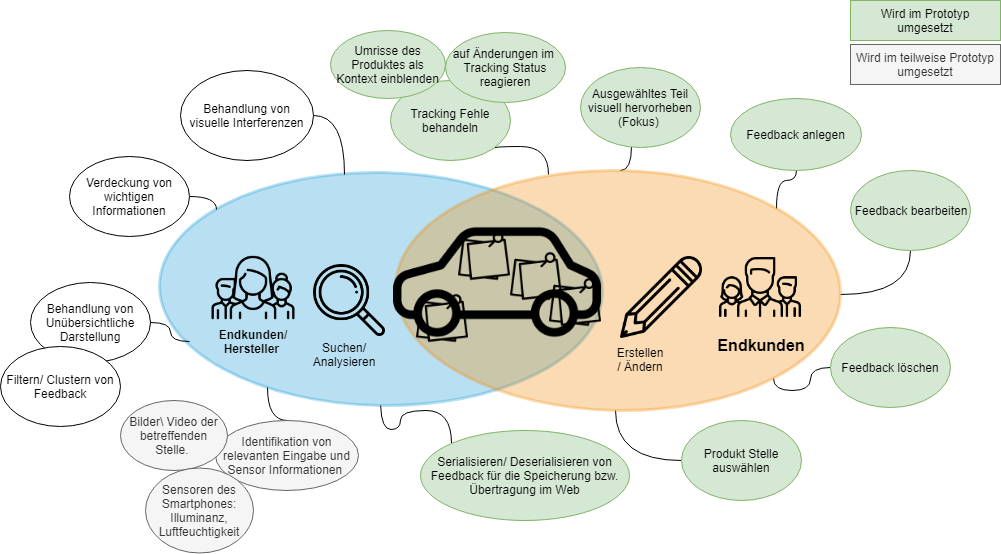
\includegraphics[width=1.0\textwidth]{resources/conception/SystemSkizze.png}
	\caption{Abstrakte Skizze des Gesamtsystems \\Quelle: Eigene Darstellung}
	\label{img:sysstem_sketch}
\end{figure}

Dieses Skizze sollte die Projektidee begreifbarer machen und als grobe Orientierung bei der Anforderungsanalyse dienen.

\section{Anforderungsanalyse}\label{anforderungsanalyse}

Als Grundlage für die Anforderungsanalyse wurde ein Kreativ Workshops durchgeführt. Das Ziel dieses Workshops war, die im Kapitel \ref{CapterFundamentals} Abschnitt \ref{UsaEng} beschriebenen Schritte des Usability Engineering Lifecycle nach Nielsen umzusetzen.   

% Vorbereitung
Das Workshop fand, am Fraunhofer IPK in Berlin statt und es nahmen fünf Teilnehmer teil. %Füge noch Informationen zu den Teilenehmer hinzu.

Zur Vorbereitung wurde in einem zuvor für diesen Workshop gebuchten, Besprechungsraum, einzelne Stationen für die am Workshop durchzuführenden Aktivitäten vorbereitet.\footnote{z.Bsp.: Aufstellung eines Pinnwand für die Erstellung eines Affinitätsdiagramms, Abbildungen von Personen für die Erstellung von Personas usw.} Zunächst wurden die Teilnehmer begrüßt und für deren Teilnahme am Workshop bedankt. 
Anschließend wurde der Anlass und der Ablauf des Workshop vorgestellt. 

%Durchführung
Mit Hilfe einer kurzen Präsentation wurde die Projektidee vorgestellt und anhand einer groben Skizze des zu konzipierenden Systems (Abbildung \ref{img:sysstem_sketch}) verdeutlicht. 
Anschließend fand eine Frage- Antwort Runde statt, welches den Teilnehmern die Möglichkeit gab, Rückfragen zu stellen. Somit sollte sichergestellt werden, dass die Projektidee von 
allen Teilnehmer verstanden wurde. 

Nach Vorstellung der Projektidee fand ein Brainstorming statt, dessen Ergebnis in einer Affinitätsdiagramm festgehalten wurden. Dieses diente als Grundlage für die Erstellung von Nutzerprofilen. 
\footnote{Im gewöhnlichen Vorgang für die Erstellung von Affinitätsdiagramme, schreiben Teilnehmer Ideen auf Kärtchen, welche zunächst unsortiert auf ein Pinnwand geheftet werden. 
Anschließend werden die Ideen, gemeinsam besprochen und in Gruppen bzw. Untergruppen sortiert. In dem stattgefundenen Workshop wurden diese Gruppen jedoch im voraus vorgegeben.}

Es sollten Ideen für die Beantwortung folgender Fragen zusammengetragen werden: 

\begin{itemize}
	\item Wer sind die Nutzer (Rolle, Erfahrungsstand,  Lebensstil/ Lebenskontext)?
	\item Was sind aktuelle Problemlösungsstrategien der Nutzer?
	\item Was sind die Ziele der Nutzer?
	\item Wo liegen die Schmerzpunkte mit aktuellen Lösungstretarien?
\end{itemize}\label{list:AffiDiagramm}

Es wurde eine Zeitbegrenzung von 15 Minuten Zeit vorgegeben, innerhalb welcher Ideen zu den, oben genannten Fragen, auf Kärtchen aufgeschrieben wurde.
Folgende Ideen sind dabei entstanden welche im nächsten Schritt als Orientierung für die Erstellung von Personas dienten\footnote{Eine Abbildung des entstandenen Affinitätsdiagramm befindet sich im Anhang [Referenz darauf]}: 

\vspace{2mm}
\textit{Wer sind die Nutzer:} 
Technik Nerd, Produkt Entwickler, Werbeagentur, Unzufriedene, Unerfahrene, Gewerbliche Nutzer/ Laborpersonal, Endkunde, Qualitätsprüfung eines Produkts (Vorgesetzter), Lagerpersonal

\vspace{2mm}
\textit{Aktuelle Problemlösungsstrategien:} 
Email, Chat, Web-Portale, Telefonsupport, Vergleich von Käuferbewertungen

\vspace{2mm}
\textit{Ziele der Nutzer: } 
Nächstes Produkt sollte besser sein, Eigenes Design, Fehleranfälligkeit beseitigen, Informationen vor dem Kauf, Hilfreiche Bewertungen finden und verstehen, Ersatzteile beschaffen, Lösungen aus dem Nutzerkreis bereitstellen, Infos in Form: Kurzer Beschreibungen/ Kontakt Informationen des Verantwortlichen, Anleitungen, Reklamation Technischer Dokumentationen (Montageanleitung)

\vspace{2mm}
\textit{Wo liegen die Schmerzpunkte: } 
Komplizierte Beschreibung der Umgebung/ Use-Case, Zustand der Bearbeitung unbekannt, Fehlerbehebung meines Produktes, Produkt wird nicht wie vorgesehen (geplant) genutzt und funktioniert daher nicht richtig (Vorstellung eines möglichen neuen Anwendungsfalles), Lange Wartezeiten auf Antwort, Bessere Kommunikation zwischen Abteilungen

\textbf{Personas}:
%Durchführung %Aufbau / Einleitung / Affinitätsdiagram / Personas / Szenarien
Im nächsten Schritt wurden auf Grundlage der im  Affinitätsdiagramm festgehaltenen Stichpunkte, Personas erstellt. Diese repräsentieren, stellvertretend die Ziele der 
Nutzer des zu konzipierenden Systems.

Es wurden Bilder von Personen unterschiedlicher Alter und Geschlecht auf dem Boden ausgelegt. Die Bilder zeigten die Personen in jeweils unterschiedlichen Situationen, 
sodass möglichst individuelle Eigenschaften ausgemacht werden konnten. Es fand eine kurze Diskussion statt indem, Abbildungen von Personen ausgewählt wurden welche, realistische 
Nutzer für das zu konzipierende System darstellen. Anschließend wurden den Personas fiktive Namen gegeben und die Begriffe aus dem Affinitätsdiagramm in gemeinsamer Abstimmung den 
einzelnen Personen zugeordnet. 

Auf diese weise wurde in Anlehnung an das von \citeauthor{DieterSchmalstieg2016} in \cite[S.~57]{DieterSchmalstieg2016} vorgestellte Beispiel, fünf unterschiedliche Personas erstellt (Tabelle \ref{tab:personas}, Eine vollständige Beschreibung der Personas befindet sich im Anhang \ref{anhangA}). Die Personas, Felix, Timo und Svenja sind für die Implementierung des Prototypen besonders bedeutsam. Diese Personas werden das System nutzen um Feedbacks zu erstellen, 
zu bearbeiten und zu löschen. Die Personas Magitta und Flo dienen dazu um ein Verständnis für das zu konzipierende Gesamtsystem aufzubauen in welchem sich der Prototyp einfügen soll. Diese werden vorwiegend die Artefakte 
welche durch das System entstehen nutzen. 

\begin{table}[htbp]
	\caption{Zusammenfassung der Personas}
		\begin{tabular}{|l|l|l|}
			\hline
			 \textbf{Name} & \textbf{Rolle}& \textbf{Ziele und Bedürfnisse}\\
			\hline
			\textbf{Timo} &  Produktentwickler & \makecell[l]{*Oft sind komplizierte Anwendungsfälle schwer zu beschreiben.\\ *Produktbezogene Beschreibungen bei welchen Bezug zu \\spezifischen Stellen  am Produkt\\ genommen werden muss\\ oft von anderen nicht verstanden.} \\
			\hline
			\textbf{Svenja} & Auszubildende & * \makecell[l]{Möchte dass es besonders einfach und unkompliziert benutzbar ist.}\\
			\hline
			\textbf{Felix} & Zahnarzt &  \makecell[l]{* Möchte dass seine Laborgeräte \\einwandfrei funktionieren.\\ * Möchte bei technischen Problemen schnelle\\ * Rückmeldung vom Hersteller. \\Qualität der Produkte\\ haben einen Einfluss auf sein Betrieb.} \\
			\hline
			\textbf{Magitta} & Produktmanagerin & \makecell[l]{* Möchte die Produkte\\ ihres Unternehmens zu verbessern.\\ * Wo liegen die Schwächen? Wo die Stärken?\\* Wie werden die Produkte von \\den Kunden wahrgenommen?}\\
			\hline
			\textbf{Flo} & Daten Analyst & \makecell[l]{* Möchte aus Daten Wissen generieren.\\ * Möchte über eine Schnittstelle präzise\\ Kundenfeedbacks zu Produkten erheben\\ um aus diesen Erkenntnisse zu generieren}\\ 
			\hline
		\end{tabular}
	\label{tab:personas}
\end{table}

\textbf{Szenarien}:

Basierend auf den entworfenen Personas, wurden im nächsten Schritt Ist-Szenarien beschrieben (Siehe Anhang: \ref{anhangA} Abschnitt Ist-Szenarien). Mit diesen wurden aktuelle Problemlösungsstrategien der Personas Timo, Felix und Svenja im jeweiligen Anwendungskontext beschrieben. Dabei wurden besonders die Schmerzpunkte der aktuellen Lösungstretarien betont. Die Ist-Szenarien wurden hinsichtlich mögliche Verbesserungen mit einer neuen Lösung analysiert und im weiteren Schritt wurden Soll-Szenarien entwickelt (Siehe Anhang \ref{anhangA} Abschnitt Soll-Szenarien). 

Die Soll-Szenarien beschreiben, in welchem Kontext sowie unter welchen Bedingungen die Anwendung verwendet wird um die Aufgabe, ein Feedback an einem physischen Produkt abzugeben. 
Die beschriebenen Soll-Szenarien beinhalten Beschreibungen für Funktionen welche nicht im Prototypen enthalten sein werden. Diese dienen dazu um ein Verständnis dafür aufzubauen zu können, wie sich der Prototyp in ein Gesamtsystem mit diesen Funktionen einfügen wird. 

Funktionen welche in den Ist-Szenarien beschrieben werden jedoch nicht Teil des Prototypen sein werden: 

\begin{itemize}
\item{Anmeldevorgang} 
\item{Produktauswahl} 
\item{Feedbacks von anderen Nutzern auf dem Produkt sehen}
\item{Versand von Informationen an den Hersteller}
\end{itemize}

%Svenja. Praktisch, schnell. 
%Felix Vorgang zum Auswählen eines teils + Wunsch äußern dass Rückmeldung vom Hersteller erwünscht ist.
%Timo Kategorien zum Auswählen

\textbf{User Stories}:

Auf Grundlage der Soll-Szenarien, wurden im nächsten Schritt User Stories beschrieben welche im Prototypen implementiert werden: 

%\begin{center}
	\begin{table}[htbp]
	\caption{User Stories}
	\resizebox{\textwidth}{!}{
	\begin{tabular}{ | c | c | c |c |c |}
		\hline
		\thead{Nr.} & \thead{Als} & \thead{abgeleitet \\ aus \\ Persona} &	\thead{möchte ich} & \thead{damit} \\
		\hline
		10 &  \makecell{Endkunde} & \makecell{Timo} & \makecell{neue Anwendungsfälle \\direkt am Produktteil\\ beschreiben können} &  \makecell{ich bei meiner Beschreibung\\ implizit ein Bezug\\
			zu einer bestimmten\\ Stelle am Produkt\\ herstellen kann.} \\
		\hline
		20 &  \makecell{Endkunde} & \makecell{Timo} & \makecell{Ergänzende Anleitungen direkt\\ am  Produktteil\\ oder Stellen ansehen können} &  \makecell{ich mir ergänzende Bemerkungen \\und Anleitungen
			direkt an der \\ betreffenden Stelle ansehen kann.
} \\
		\hline
		21 &  \makecell{Endkunde} & \makecell{Timo} & \makecell{Fragen von anderen Kunden \\ am  betreffenden Produktteil\\ oder Stellen ansehen können} &  \makecell{die Fragen\\ besser verstehen \\ und Antworten bereitstellen kann welche anderen helfen.
		} \\
		\hline
		22 &  \makecell{Endkunde} & \makecell{Timo} & \makecell{Fragen \\ am  betreffenden Produktteil\\ oder Stellen beschreiben können} &  \makecell{die Fragen von anderen Kunden \\besser verstanden werden und Antworten und ich schneller Antworten erhalte.
		} \\
		\hline
		30 &  \makecell{Endkunde} & \makecell{Timo} & \makecell{Anleitungen zu spezifischen\\ Stellen am Produkt \\beschreiben können} &  \makecell{mir die Bezugnahme zu der\\ betreffenden Stelle
			am Produkt\\ erleichtert wird und meine \\Anleitungen
			verständlicher \\für andere werden.} \\
		\hline
		31 &  \makecell{Endkunde)}  & \makecell{Svenja, \\ Timo, \\ Felix} & \makecell{ein bestimmtes Teil an einem\\
			physischen Produkt auswählen\\
			können
} &  \makecell{ich bezugnehmend auf das ausgewählte\\ Teil
			Aktionen ausführen kann.\\ (z. B.: eine
			Rückmeldung abgeben)}\\
		\hline
		32 &  \makecell{Endkunde}  & \makecell{Svenja, \\ Timo, \\ Felix} & \makecell{eine von mir abgegebenes\\
			Feedback auswählen können,} &  \makecell{damit ich dieses Feedback oder den\\
			löschen kann}\\
		\hline
		33 &  \makecell{Endkunde}  & \makecell{Svenja, \\ Timo, \\ Felix} & \makecell{die Beschreibung auf einer von mir\\
			abgegebenes Feedback verändern\\
			können} &  \makecell{ich eine Nachträgliche Korrektur oder Ergänzung\\
			vornehmen zu kann.
}\\
		\hline
		34 &  \makecell{Endkunde}  & \makecell{Svenja, \\ Timo, \\ Felix} & \makecell{den Bezugspunkt (Produktteil oder\\
			bestimmte Stelle auf einem\\
			Produktteil) auf die, ein von mir\\
			erstelltes Feedback sich bezieht\\
			ändern können
} &  \makecell{ich eine Nachträgliche Korrektur oder Ergänzung\\
			vornehmen zu kann.
}\\
		\hline
		35 &  \makecell{Endkunde}  & \makecell{Svenja, \\ Timo, \\ Felix} & \makecell{ein von mir erstelltes Feedback\\
			löschen können} &  \makecell{ich eine obsolete, redundante oder versehentlich\\
			erstellte Rückmeldung wieder entfernen kann.}\\
		\hline
		40 &  \makecell{Endkunde}  & \makecell{Svenja} & \makecell{schnell und unkompliziert\\
			Feedbacks zu Teile od. Stellen am Produkt\\
			abgeben können.} &  \makecell{ich auch Feedbacks beiläufig abgeben kann.}\\
		\hline	
		50 &  \makecell{Endkunde}  & \makecell{Svenja, \\ Timo, \\ Felix} & \makecell{Bewertungen zu ein\\
			Produkt, an der Betreffenden Stelle am\\ Produkt ansehen können} &  \makecell{ich mich vor dem Kauf eines Produktes genauer\\
			erkundigen kann, und mir vor allem, die für mich
			wichtigen stellen am \\Produkt besser beurteilen
			kann
}\\
		\hline	
		60 &  \makecell{Endkunde}  & \makecell{Svenja, \\ Timo, \\ Felix} & \makecell{Kontaktinformationen zu\\
			Verantwortlichen Personen sehen\\
			können.} &  \makecell{ich direkt Kontakt zu dieser Person aufnehmen\\
			kann.}\\
		\hline	
		70 &  \makecell{Geschäftskunde\\(gewerblich\\nutzender\\Endkunde)}  & \makecell{Felix} & \makecell{möchte ich den Wunsch äußern\\
			können, dass der Hersteller über mein\\
			Feedback informiert wird} &  \makecell{ich sichergehen kann dass mein Feedback\\
			zeitnah vom Hersteller wahrgenommen wird}\\
		\hline	
		80 &  \makecell{Geschäftskunde\\(gewerblich\\nutzender\\Endkunde)}  & \makecell{Felix} & \makecell{bei Abgabe eines Feedback,\\ den
			Einfluss auf mein Geschäft\\ oder Anwendungsfall \\
			beschreiben können} &  \makecell{ich dem Hersteller des Produktes\\ ein besseres Verständnis über den Ausmaß ermöglichen\\ kann und dieser den im Feedback\\ entsprechend beurteilen und priorisieren kann }\\
		\hline	
\end{tabular}}
	\label{tab:userstories}	
\end{table}
%\end{center}

\section{Entwurf}\label{entwurf}

Im folgenden Abschnitt wird der erste Entwurf des zu entwickelnden Prototypen beschrieben. Es wird zunächst ein Papierprototyp vorgestellt welches ein Entwurf der Benutzeroberfläche darstellt. 
Anschließend werden die einzelnen Module vorgestellt welche das System besitzen wird. Anschließend werden die durch das System zu speichernden Daten in Form einer Entitätentyp festgelegt und dargestellt
sowie die Klassendiagramme für den digitalen Prototypen entworfen.  

\subsection{Low-Fidelity-Prototyp}\label{lowfi}

Die in der Anforderungsanalyse erstellten Soll-Szenarien sowie die festgelegten User Stories wurden zur Orientierung für die Gestaltung des Papierprototypen verwendet
Folgend werden die einzelnen Ansichten des entwickelten Papierprototypen vorgestellt und erläutert: 
%Es wurden Techniken 

Auf Abbildung \ref{img:pp_start} ist das Startbildschirm der Anwendung zu sehen. Auf dieser gelangt der Nutzer sobald die Anwendung gestartet wurde. 
In der Mitte des Bildschirmes wird ein Text eingeblendet, welches den Nutzer dazu auffordert, die Kamera auf das Produkt\footnote{Das Wort ``Product`` wird an dieser Stelle in der Annahme verwendet dass für das Tracking ein CAD Modell des physischen Produktes verwendet wird. Dies kann sich je nach verwendeter Tracking Methode ändern.} zu richten. Dieser Text wird eingeblendet, damit die Registrierung des Produktes stattfinden kann und ist in dieser Ansicht immer sichtbar wenn die Registrierung nicht stattfinden kann.

Auf der linken oberen Ecke des Bildschirmes befinden sich zwei Buttons mit den Aufschriften ``My Feedbacks`` und ``New Feedbacks``. Durch das klicken auf das Button ``My Feedbacks`` gelangt der Nutzer in 
das auf Abbildung \ref{fig:pplist} vorstellte Ansicht in welchem er die Möglichkeit hat die von ihm erstellen Feedbacks zu bearbeiten oder zu löschen. Klickt der Nutzer auf das Button mit der Aufschrift 
``New Feedbacks`` gelangt er in das auf Abbildung \ref{img:ppcreate} dargestellte Ansicht. In dieser ist die Anwendung in einem Modus in welcher Produktteile für die Erstellung neuer Feedback ausgewählt werden können. 

\begin{figure}[H]
	\centering
	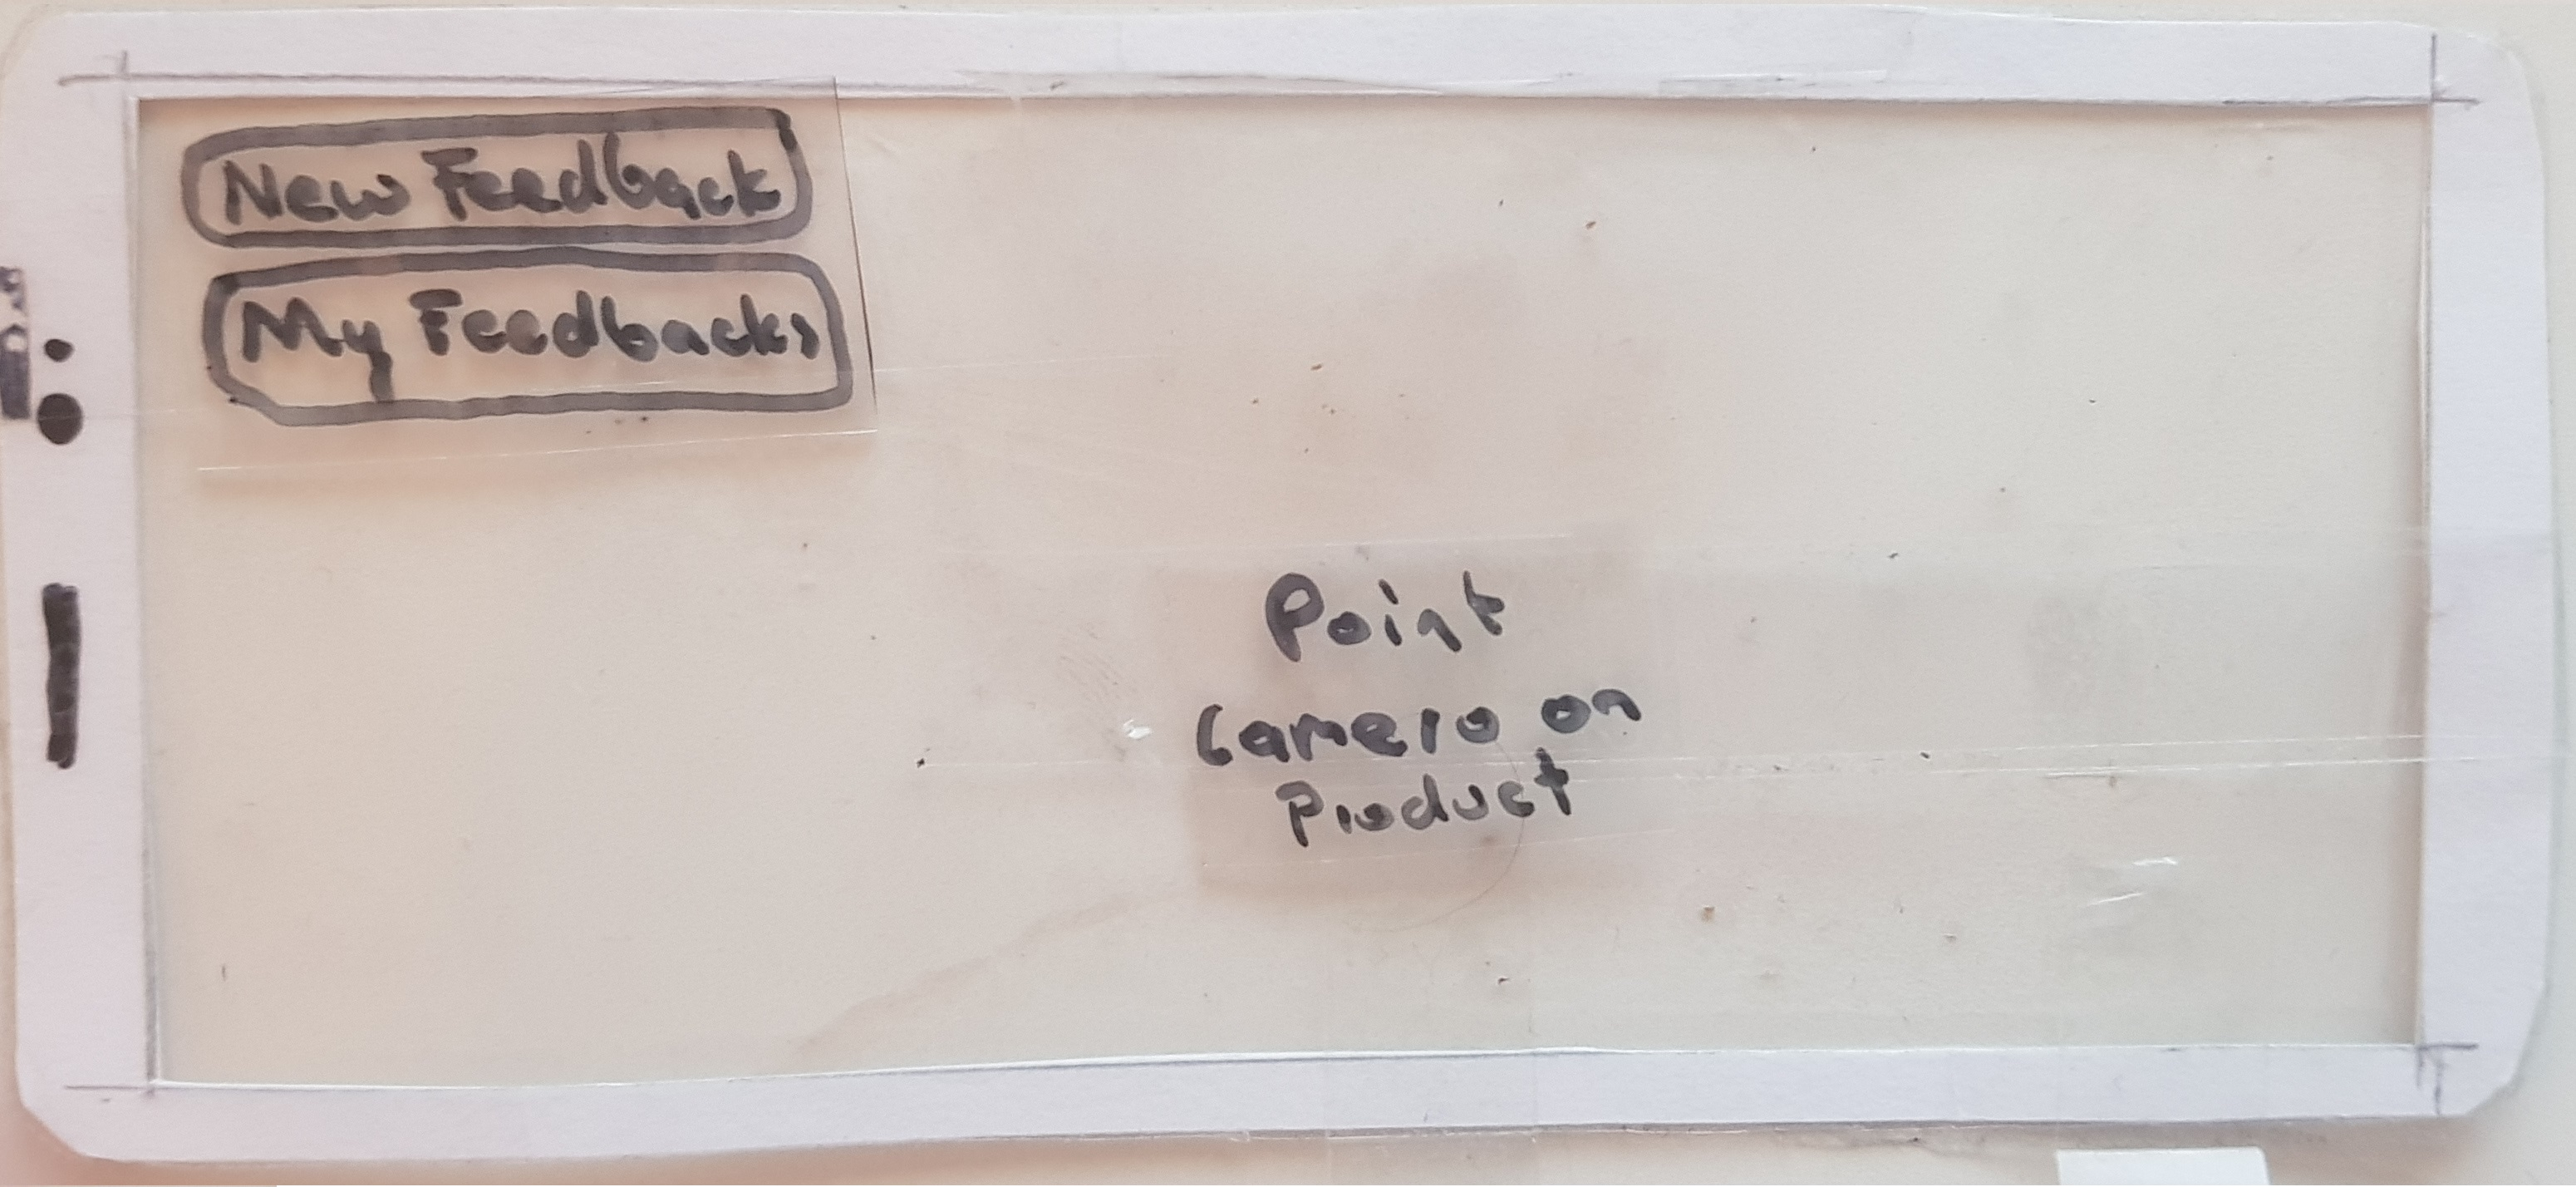
\includegraphics[width=.7\textwidth]{resources/conception/lowfi_startbildschirm.jpg}
	\caption{Papierprototyp - Startbildschirm  \\Quelle: Eigene Darstellung}
	\label{img:pp_start}
\end{figure}

Sobald die Kamera auf das Produkt gerichtet wird, findet Registrierung statt. Das heißt dass, das 3D Modell des physischen Produktes über das reale Produkt gelegt wird und dieses überlagert. 
Dieses virtuelle Modell wird durchsichtig dargestellt, sodass das reale Produkt sichtbar bleibt. Die Konturen des virtuellen Produktes jedoch sollen im Falle einer fehlerhafter Registrierung dem Anwender 
die Konturen des virtuellen Modells als Kontext zeigen.

In dieser Ansicht kann der Nutzer das Produkt durch das Bildschirm des Smartphones betrachten wobei bestehende Feedback auf dem Produkt in Form von Annotationen dargestellt werden. Die Annotationen werden mit Verbindungslinien dargestellt welches Bezugspunkt auf dem Produkt und Text Miteinander verbinden. Dies wurde auf Grundlage Forschungsergebnisse in \cite{Brandenburg2019} \cite{Polys2007} entschieden, welche feststellen dass Annotationen die mit Verbindungslinien dargestellt werden bessere Effizient in der Bearbeitung der Aufgaben aufweisen.

\begin{figure}[H]
	\centering
	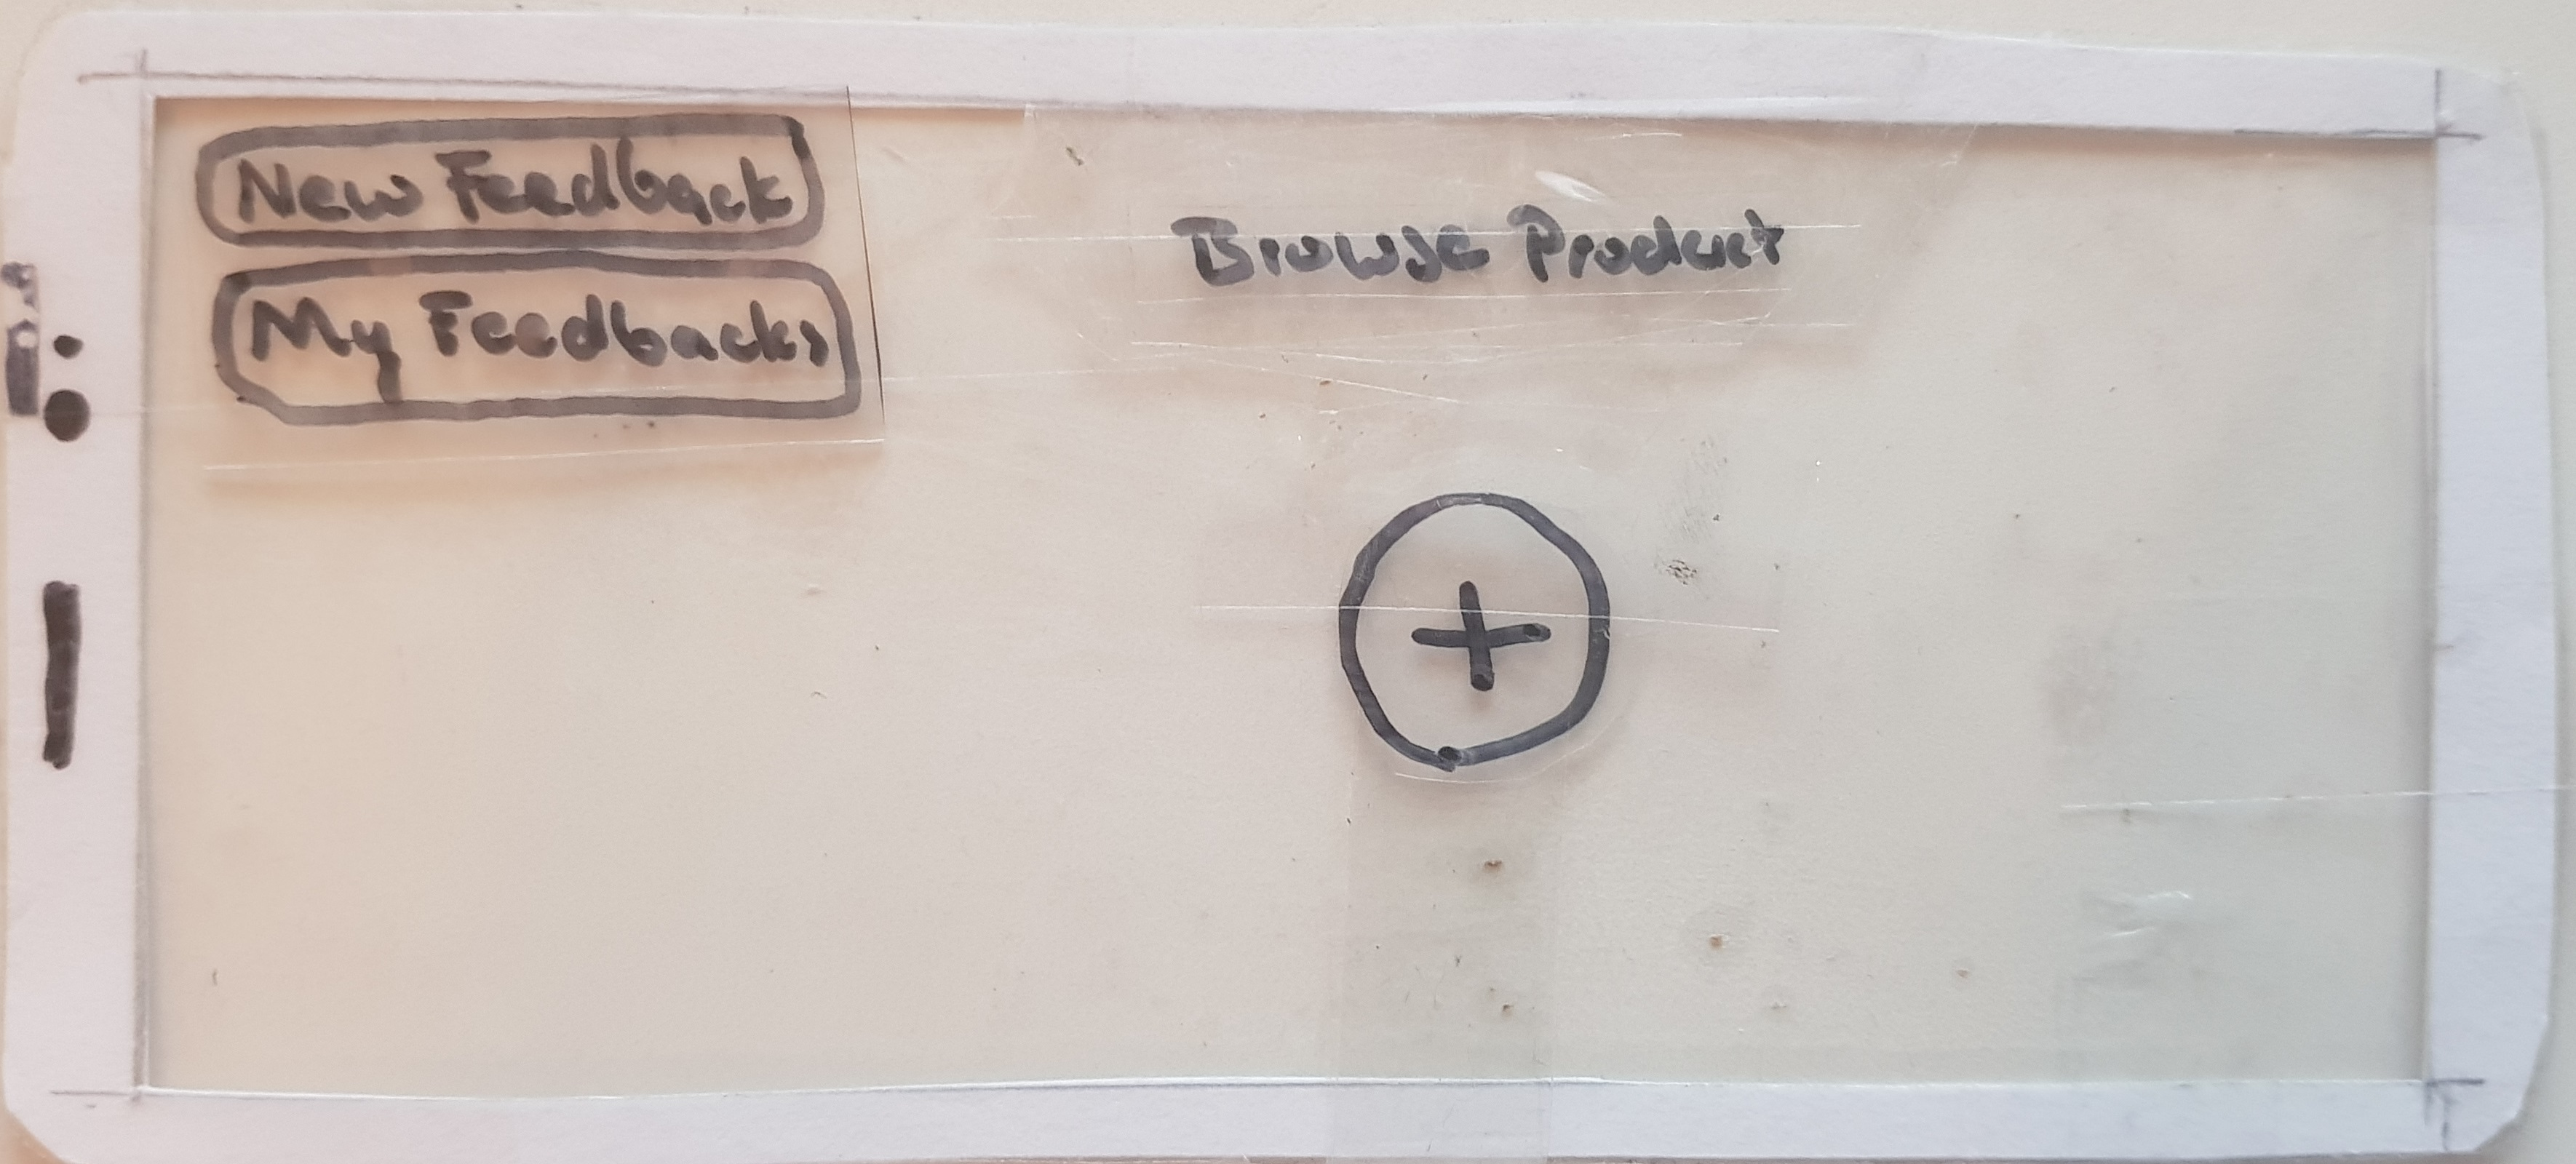
\includegraphics[width=.7\textwidth]{resources/conception/lowfi_browseOnProduct.jpg}
	\caption{Papierprototyp - Ansicht zum Suchen und Finden von Feedbacks auf dem Produkt. \\Quelle: Eigene Darstellung}
	\label{img:lowfibowseonproduct}
\end{figure}

In der auf Abbildung \ref{img:ppcreate} gezeigten Ansicht, befindet sich die Anwendung in einem Modus in welcher eine Stelle oder Produktteil für die Erstellung eines neuen Feedbacks ausgewählt werden kann. 

Um die Funktion Zeigen und Auswählen realistischer testen zu können wurde entschlossen diese als vertikale Prototypen zu implementieren und anschließend von einer kleinen Nutzergruppe testen zu lassen.
Dafür wurden die zwei von \citeauthor{Vincent2013} vorgestellten Methoden aus Kapitel \ref{anlayse_capter} Abschnitt \ref{pointer_section}: \textit{Crossfade} und \textit{Relative-Pointing} als Vorlage genommen.

Abbildung \ref{img:ppcreate} zeigt die Ansicht für die Variante \textit{Crossfade}. In dieser Ansicht wird in der Mitte des Bildschirmes ein Fadenkreuz angezeigt. Der Nutzer kann das Smarthone auf 
die Stelle oder das Produktteil richten welches er auswählen möchte. Das Produktteil welches im Visier des Fadenkreuzes ist wird farblich hervorgehoben. Auf der rechten unteren Ecke des Bilschirmes befindet 
sich ein grüner Button mit einem Häkchen. Drückt der Nutzer auf dieses Button wird die Stelle oder das Produktteil welches im Visier des Fadenkreuzes ist ausgewählt und der Nutzer gelangt in die auf Abbildung 
\ref{fig:test1} gezeigte Ansicht.

Befindet sich im Visier des Fadenkreuzes ein auf dem Produkt vorhandenes Feedback werden, anstelle des Buttons für das Anlegen von neuen Feedback die zwei Button welche auf Abbildung \ref{img:ppeditdelete}
rechte untere Ecke zu sehen sind für das Bearbeiten und Löschen dieses Feedbacks angezeigt. 

Der Vorteil dieser Methode ist, dadurch dass die Stelle zum Auswählen nicht durch die Finger des im Zeigevorgang verdeckt wird. Der Nachteil wiederum ist dass das Auswählen mehr unter em Einfluss des Zittern der 
Hände und dem Rigistrieungs-jitter unterliegt. 

Auf der linken oberen Ecke im Abbildung \ref{img:ppcreate} befindet sich ein Button mit einer Haussymbol, dieses ist dazu da um in das Startbildschirm zurück zu gelangen.

\begin{figure}[H]
	\centering
	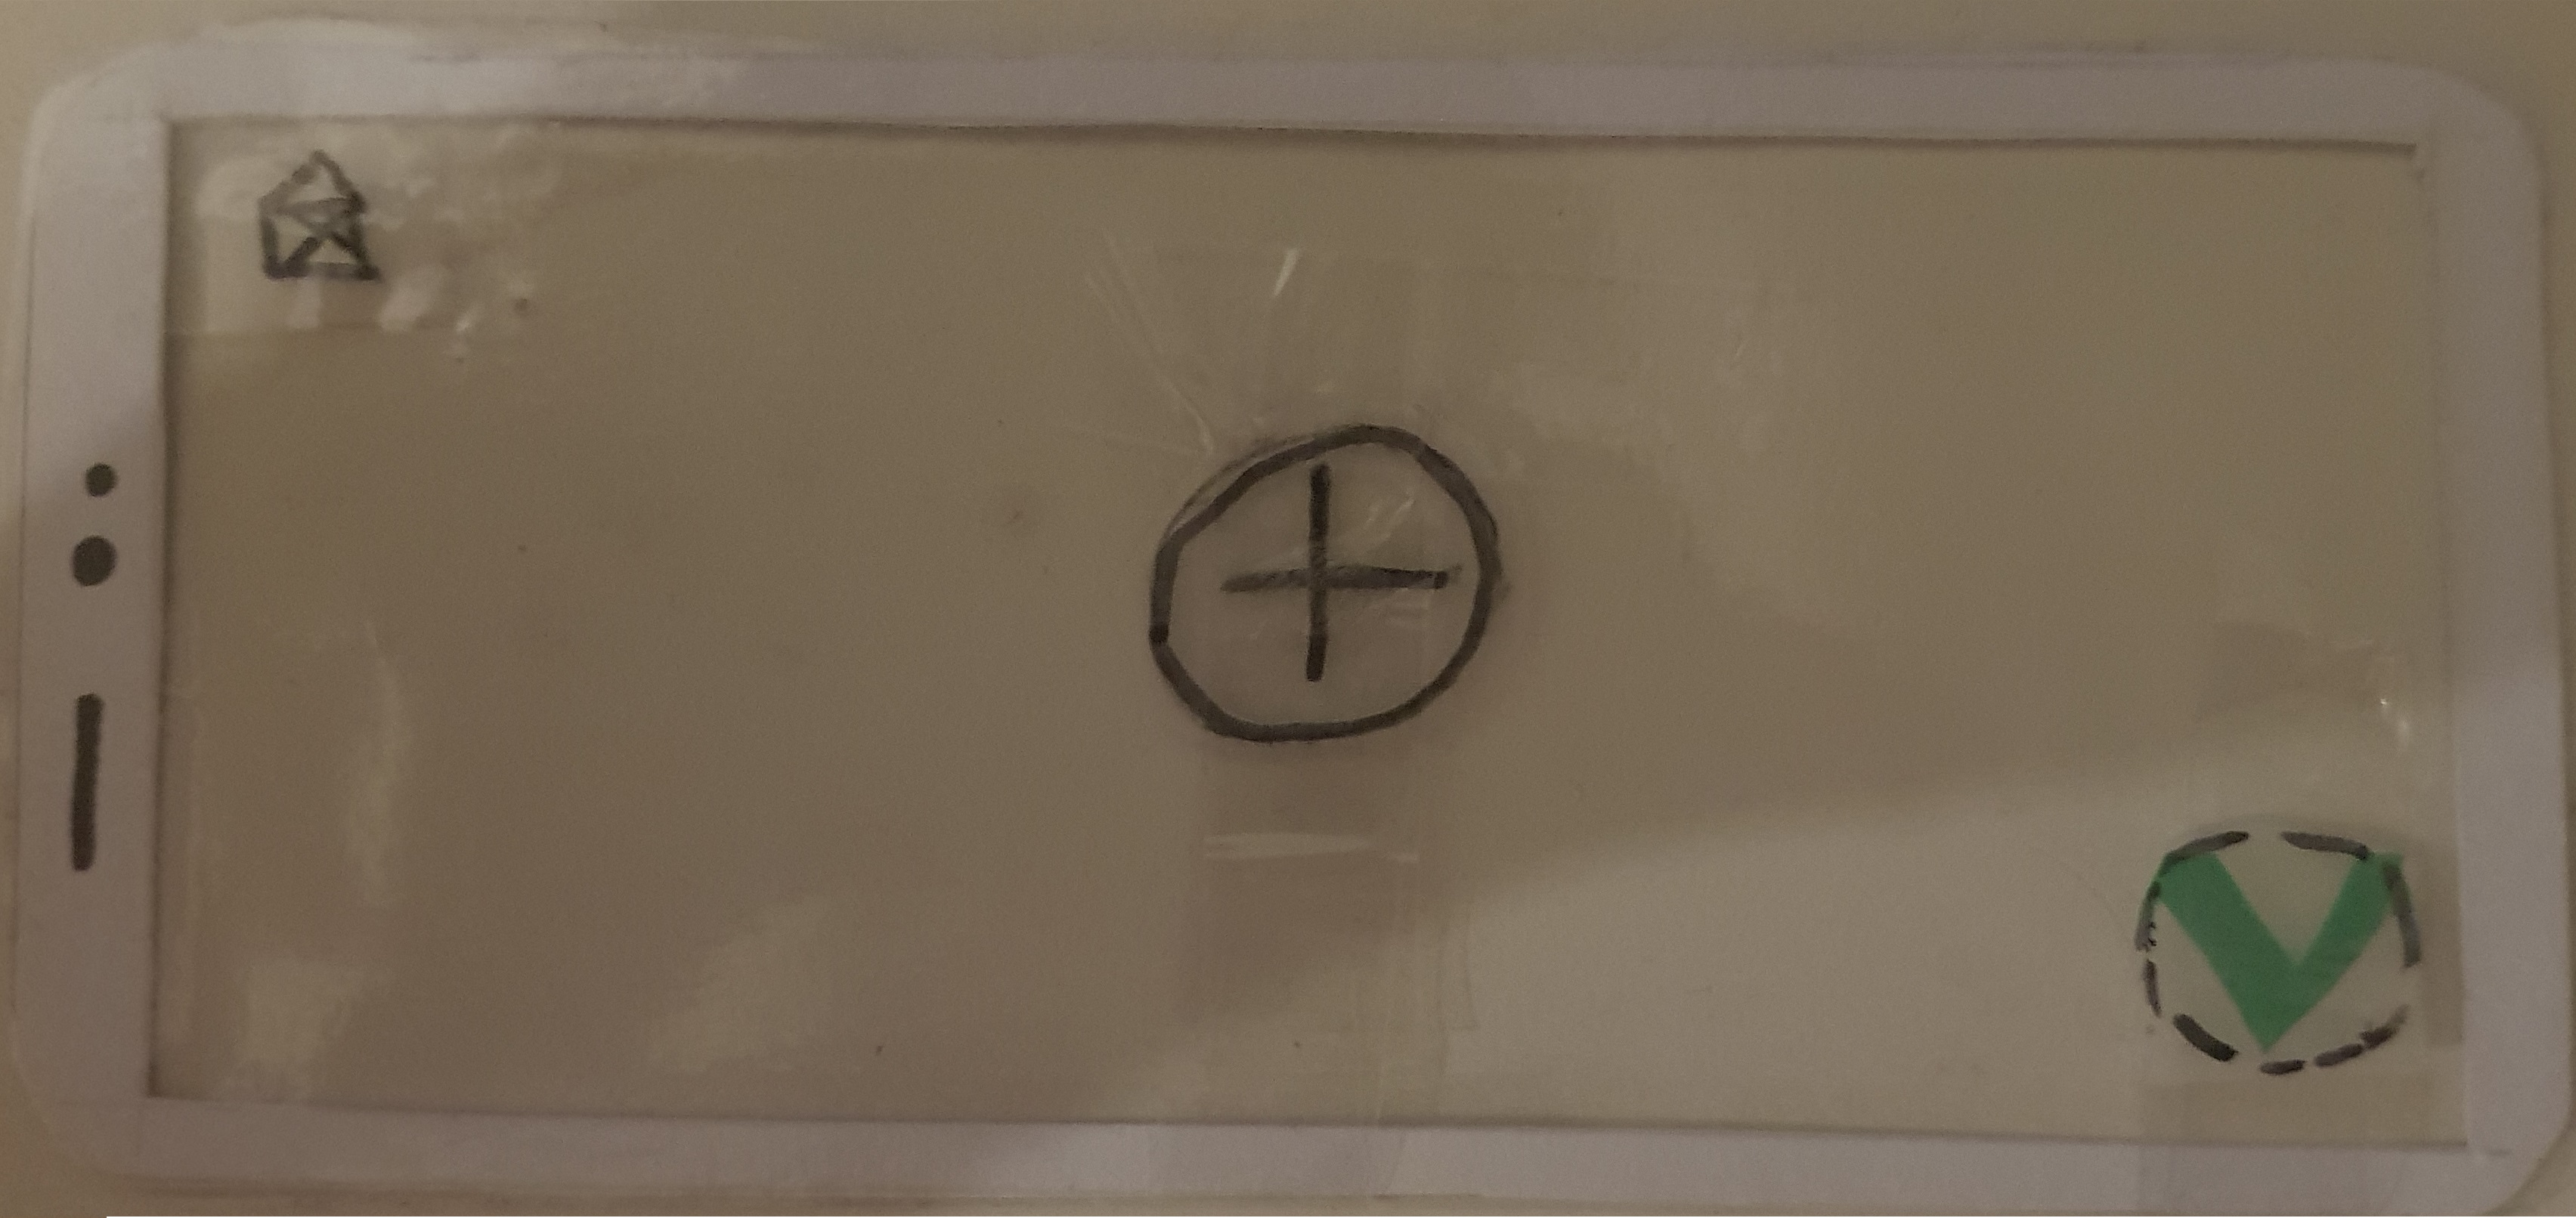
\includegraphics[width=.7\textwidth]{resources/conception/lowfi_create.jpg}
	\caption{Papierprototyp - Auswahl von Produktteil für die Erstellung eines neuen Feedback \\Quelle: Eigene Darstellung}
	\label{img:ppcreate}
\end{figure}

Abbildung \ref{img:ppeditdelete} zeigt auf der rechten unteren Ecke zwei Buttons zum Bearbeiten und Löschen von Feedback. Diese erscheinen immer dann wenn ein auf dem Produkt vorhandenes Feedback 
im von dem Fadenkreuz auf der Mitte es Bildschirmes anvisiert wird oder im Falle der Umsetzung mit der \textit{Relativ-Pointing} Methode auf das Feedback getippt wird. 

Die Icons auf diesen Buttons sind selbsterklärend. Ein Bleistift für soll das Editieren symbolisieren und eine Mülltonne das Löschen.

\begin{figure}[H]
	\centering
	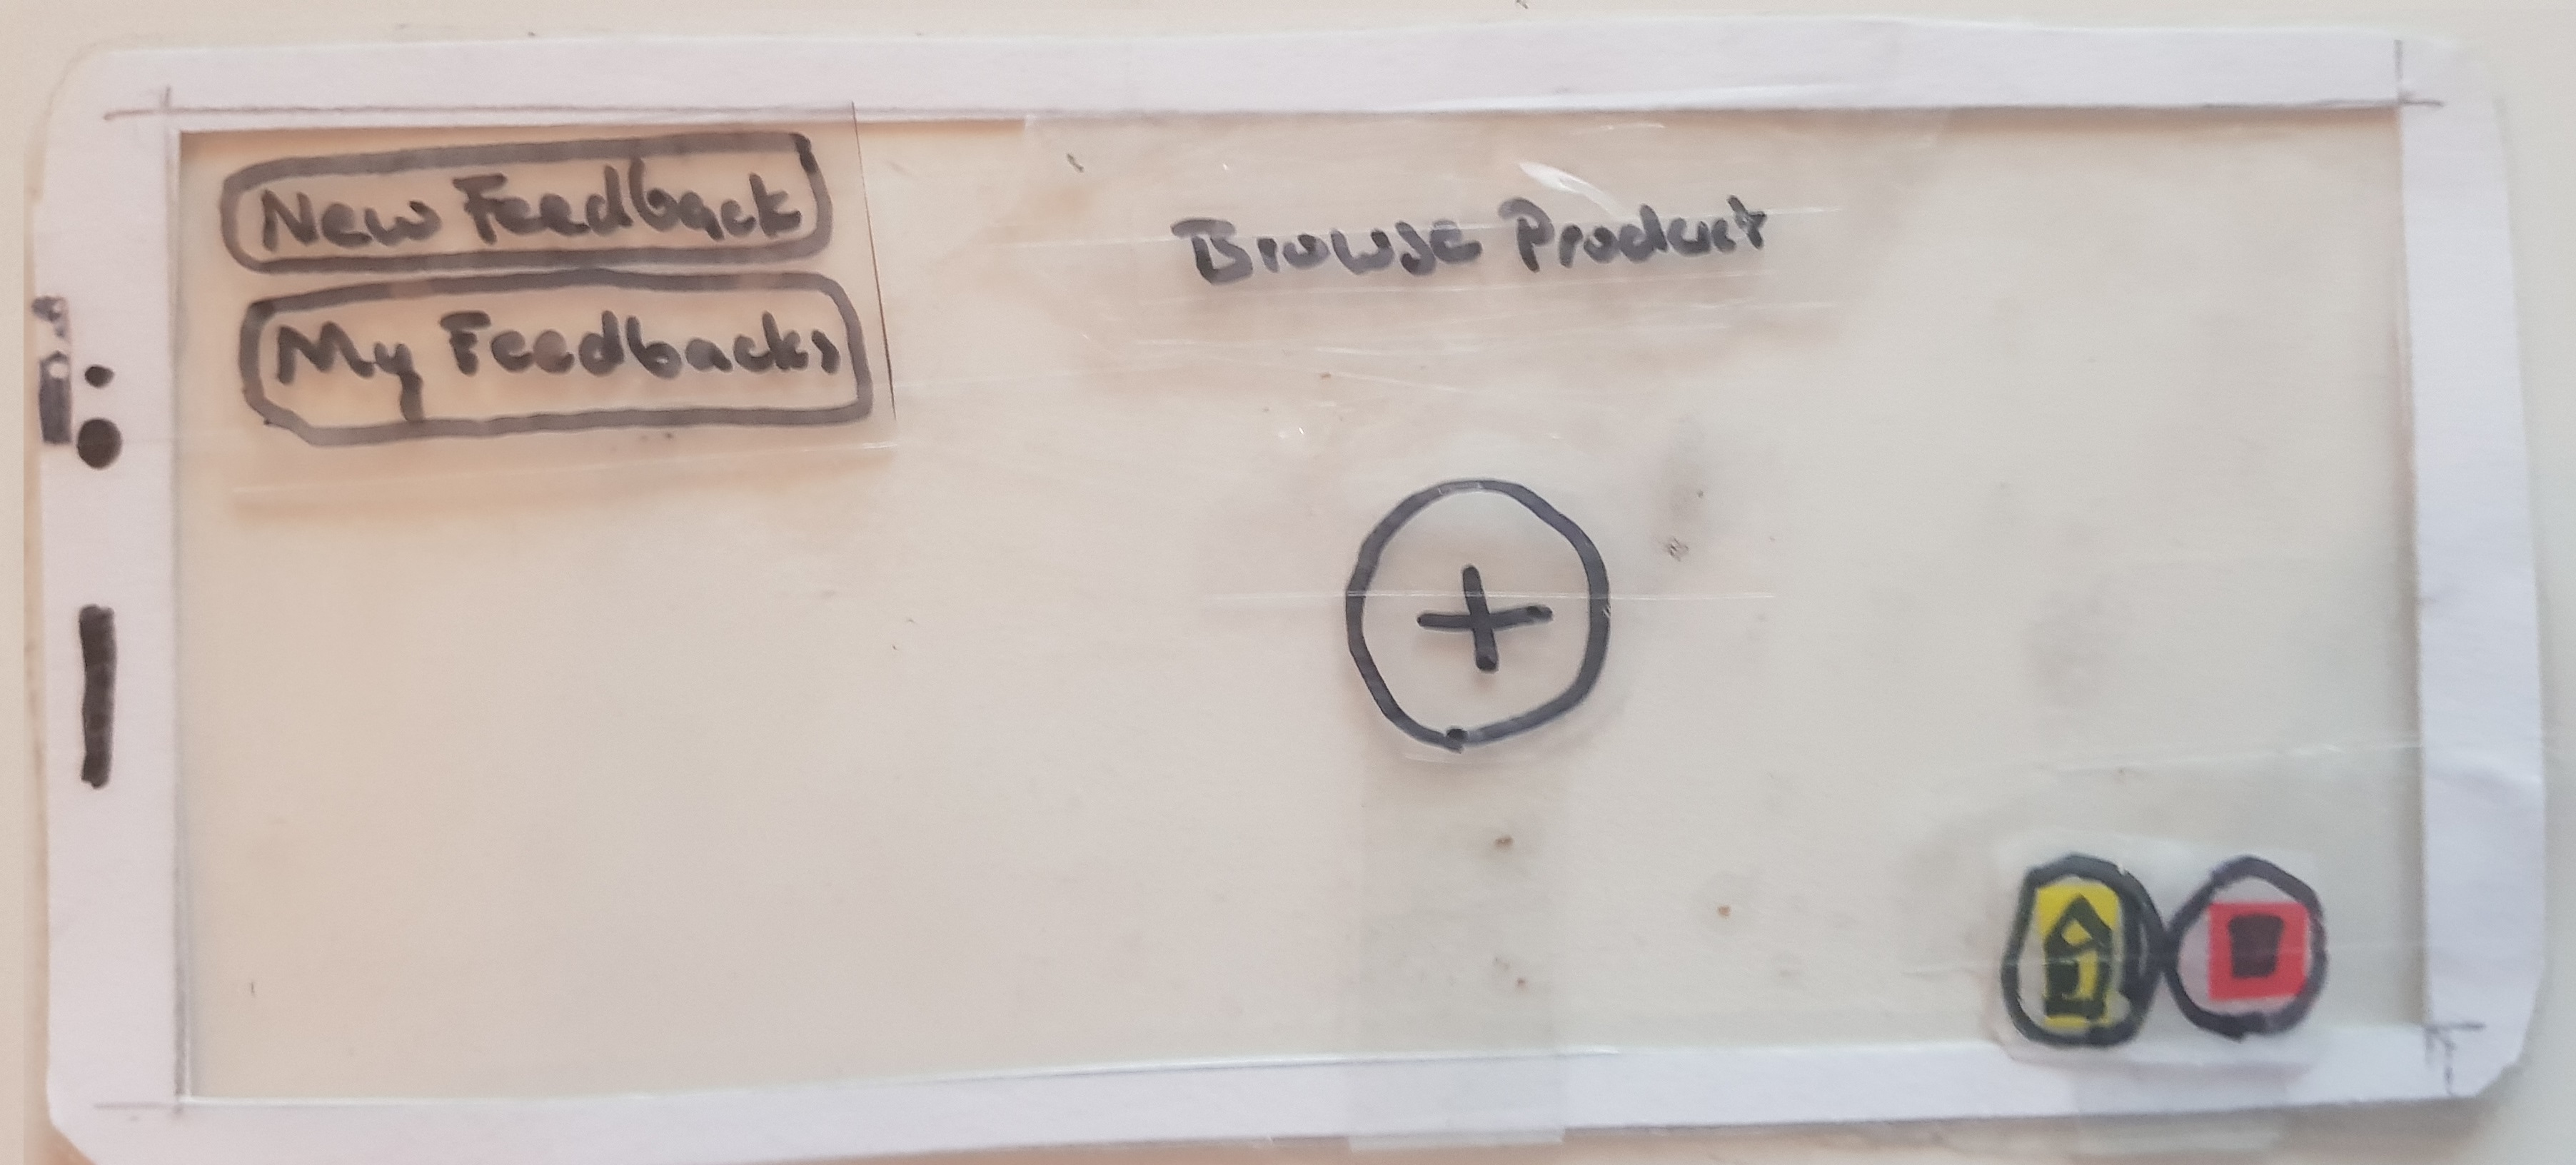
\includegraphics[width=.7\textwidth]{resources/conception/lowfi_edit_delete.jpg}
	\caption{Papierprototyp - Auswahl von Feedback auf dem Produkt für die Bearbeitung bzw. Löschung. \\Quelle: Eigene Darstellung}
	\label{img:ppeditdelete}
\end{figure}

Auf Abbildung \ref{fig:test1} ist die Formularansicht zu sehen in welcher die Nutzer nach dem Auswählen einer Stelle auf dem Produkt gelangen um Eingaben für das zu erstellende Feedback zu machen. 
Hier wurde darauf geachtet Eingabefelder zu definieren und Begrifflichkeiten zu verwenden um die Anforderungen als User Stories in Tabelle \ref{tab:userstories} festgehalten wurden abdecken zu können.

Im oberen Abschnitt des Formulars befinden sich vier Buttons für die Auswahl von einer vom Hersteller vorgegeben Kategorie. 
Dies wurde basierend an das im Kapitel \ref{anlayse_capter} Abschnitt \ref{ipi_section} von \citeauthor{Kirschner2012} in der bildzentrierten IPI Umsetzung vorgeschlagenen Entwurf (Siehe \ref{img:ipi_list_image}) entschieden.Diese Kategorien sollten den Endnutzern, insbesondere dem Persona Timo dabei helfen seine Feeeback kategorisch zu sortieren sowie beim suchen nach Feedback nach diesen zu filtern. 
Dem Hersteller sollen diese Kategorien das gewichten und analysieren der Kundenrückmeldungen unterstützen. 

Folgend werden die im Formular erhaltenen Kategorien zu den im Tabelle \ref{tab:userstories} festgehaltenen Anforderungen nach ihrer Erfüllung zugeordnet: \textit{Design} erfüllt: 40, \textit{New Use-Case} erfüllt: 10, \textit{Question} erfüllt: 21 und 22, \textit{Instruction} erfüllt: 20 und 30.

Neben der Kategorie ist befindet sich im Formular das Feld Description welches als einziges Pflichtfeld vom Nutzer ausgefüllt werden muss. 
Die Auswahl einer Kategorie ist auch Pflicht,  jedoch wird dieser mit der Kategorie ``Design`` von der Anwendung vorausgewählt. Das Genringhalten der Anzahl von Pflichtfelder beruht auf  Berücksichtigung der User Story 40. Im Feld Desctiption kann der Nutzer die Beschreibung für sein Feedback eingeben. Dieser wird nach dem Anlegen auf dem Produkt als Annotationstext sichtbar sein. 
 
Des weiteren kann eine Beschreibung eingegeben in welchem das Ausmaß auf das Geschäft oder Anwendungsfall beschrieben werden kann. 
Dieses Feld wurde unter Berücksichtigung der User Story 80 in das Formular aufgenommen nur im Fall dass eine schnelle Bearbeitung und Rückmeldung seitens des Hersteller erwünscht ist, als ein Pflichtfeld gekennzeichnet. 
Den Wusch äußern zu können eine schnelle Bearbeitung und Rückmeldung vom Hersteller zu bekommen (Tabelle \ref{tab:userstories} User Sory 70) ist im unteren Bereich des Formulars mit dem auswählen des 
Kontrollkästchens \textit{Notify Support} möglich. 

Schließlich befinden sich unten rechts ein Button womit die Eingaben bestätigt werden können und links ein Button womit der Erdstellvorgang abgebrochen werden kann. In beiden Fällen gelangt der Nutzer 
in das Startbildschirm (Abbildung \ref{img:pp_start}).

\begin{figure}[H]
	\label{tab:example}
	\centering
	\begin{minipage}{.5\textwidth}
		\centering
		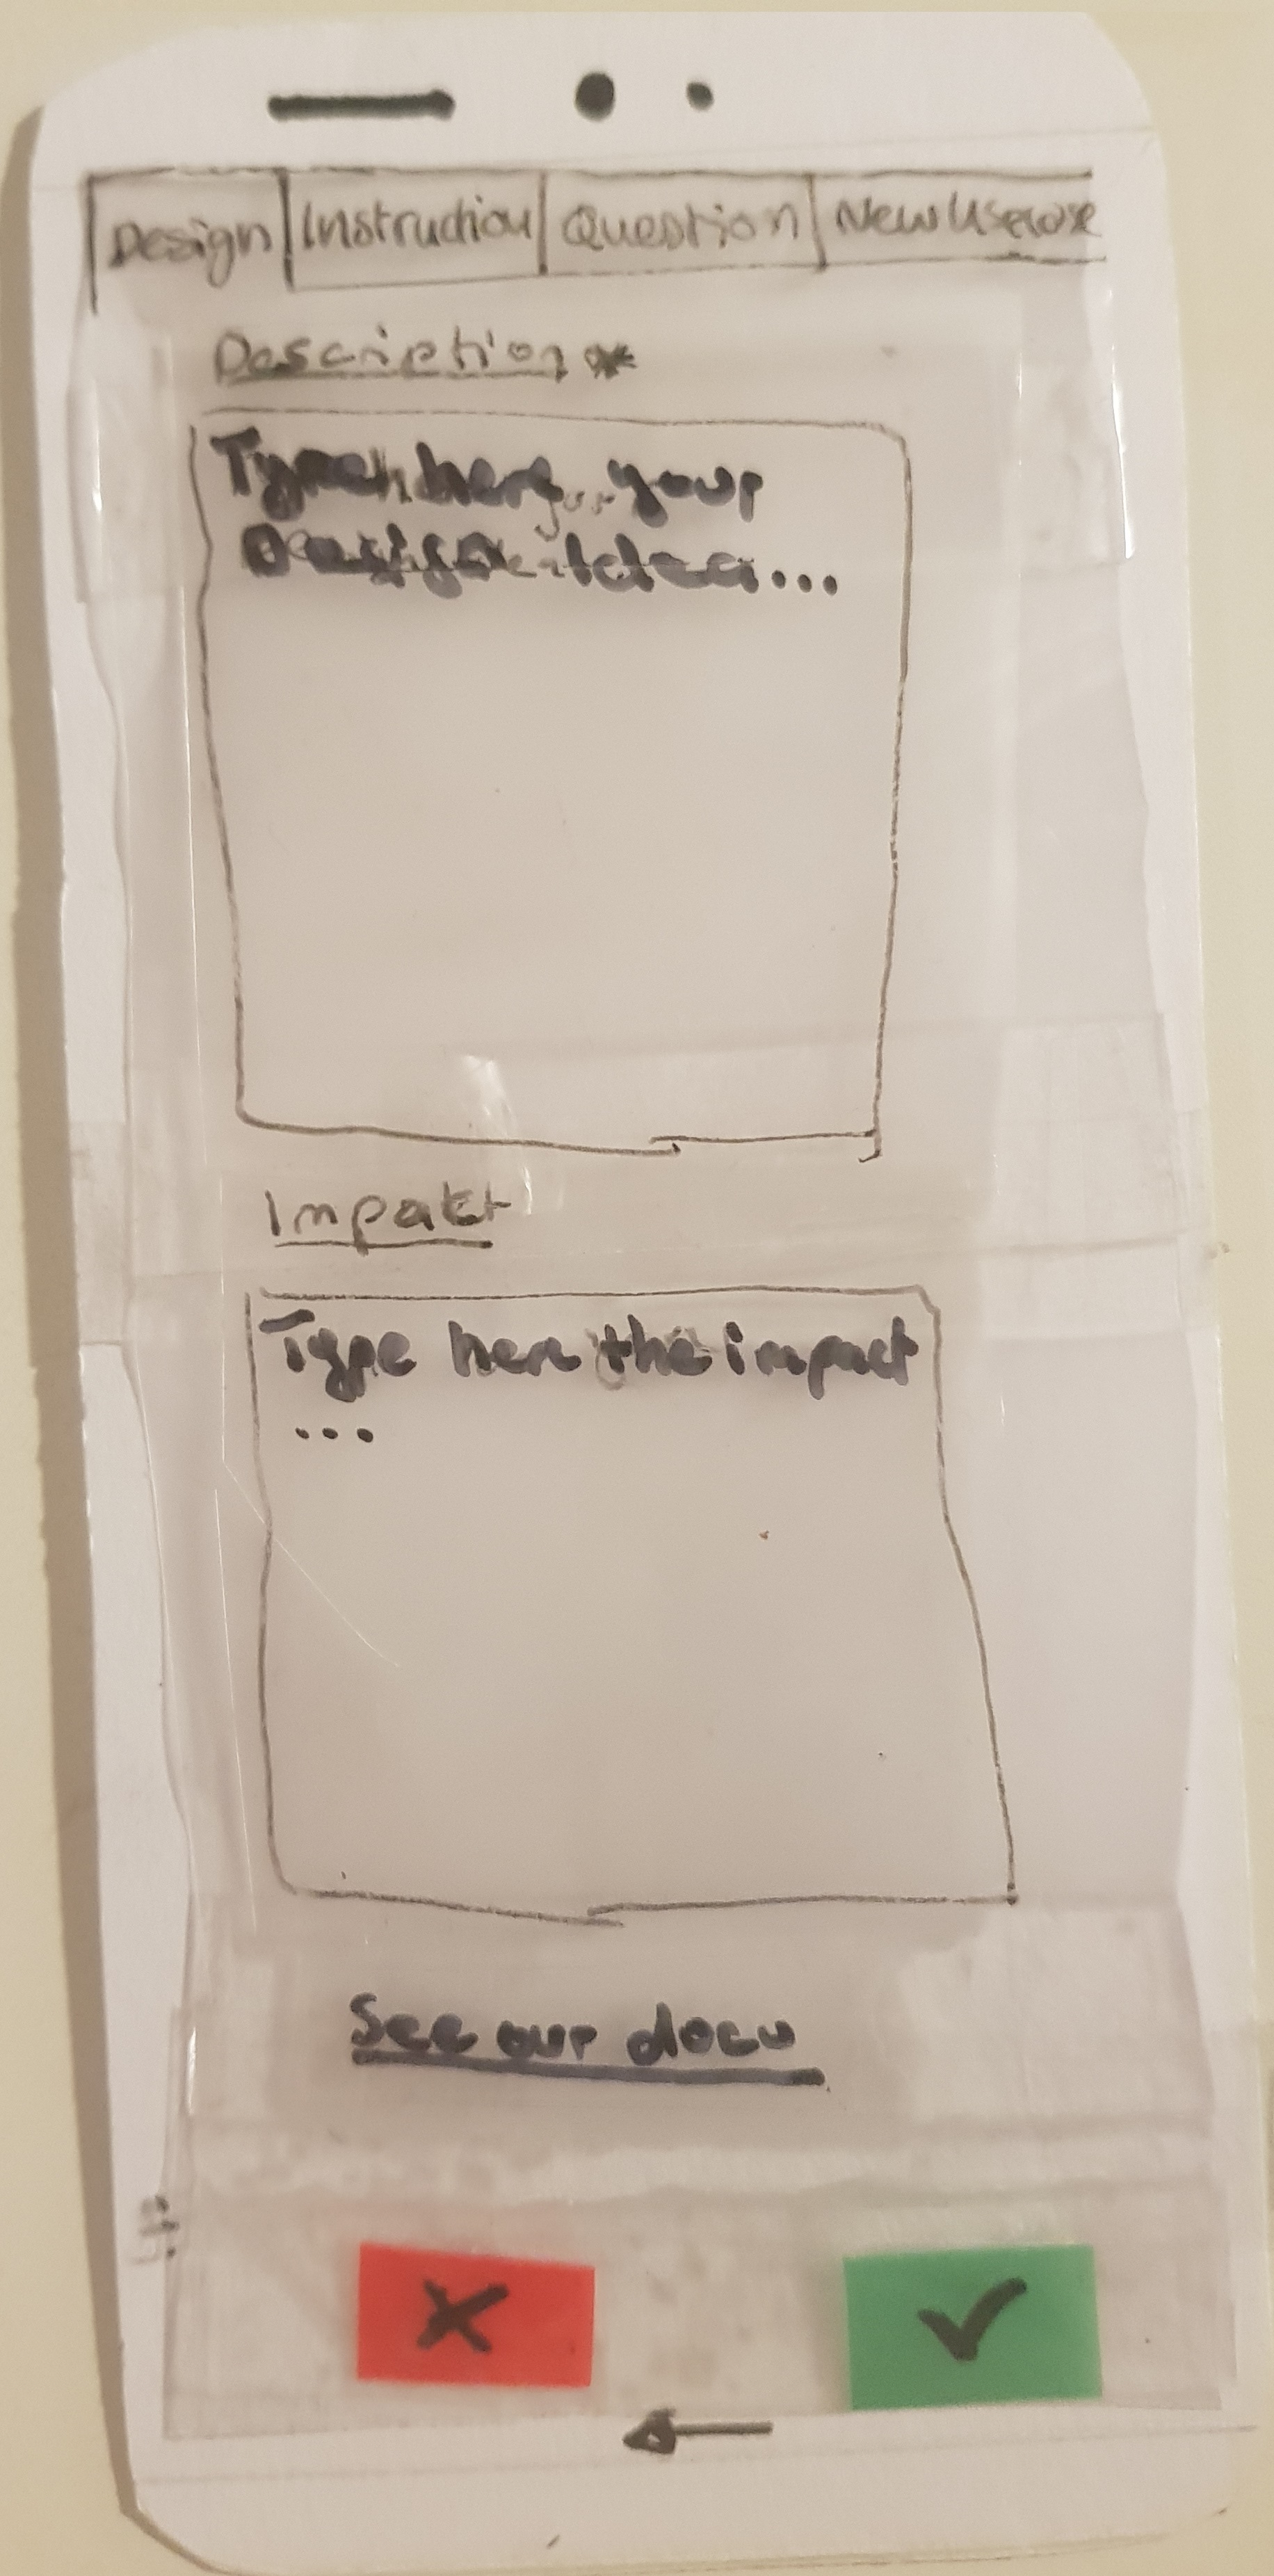
\includegraphics[width=.8\linewidth]{resources/conception/lowfi_form.jpg}
		\captionof{figure}{Papierprototyp - Eingabeformular für die \\Erstellung eines neuen Feedback.\\Quelle: Eigene Darstellung}
		\label{fig:test1}
	\end{minipage}%
	\begin{minipage}{.5\textwidth}
		\centering
		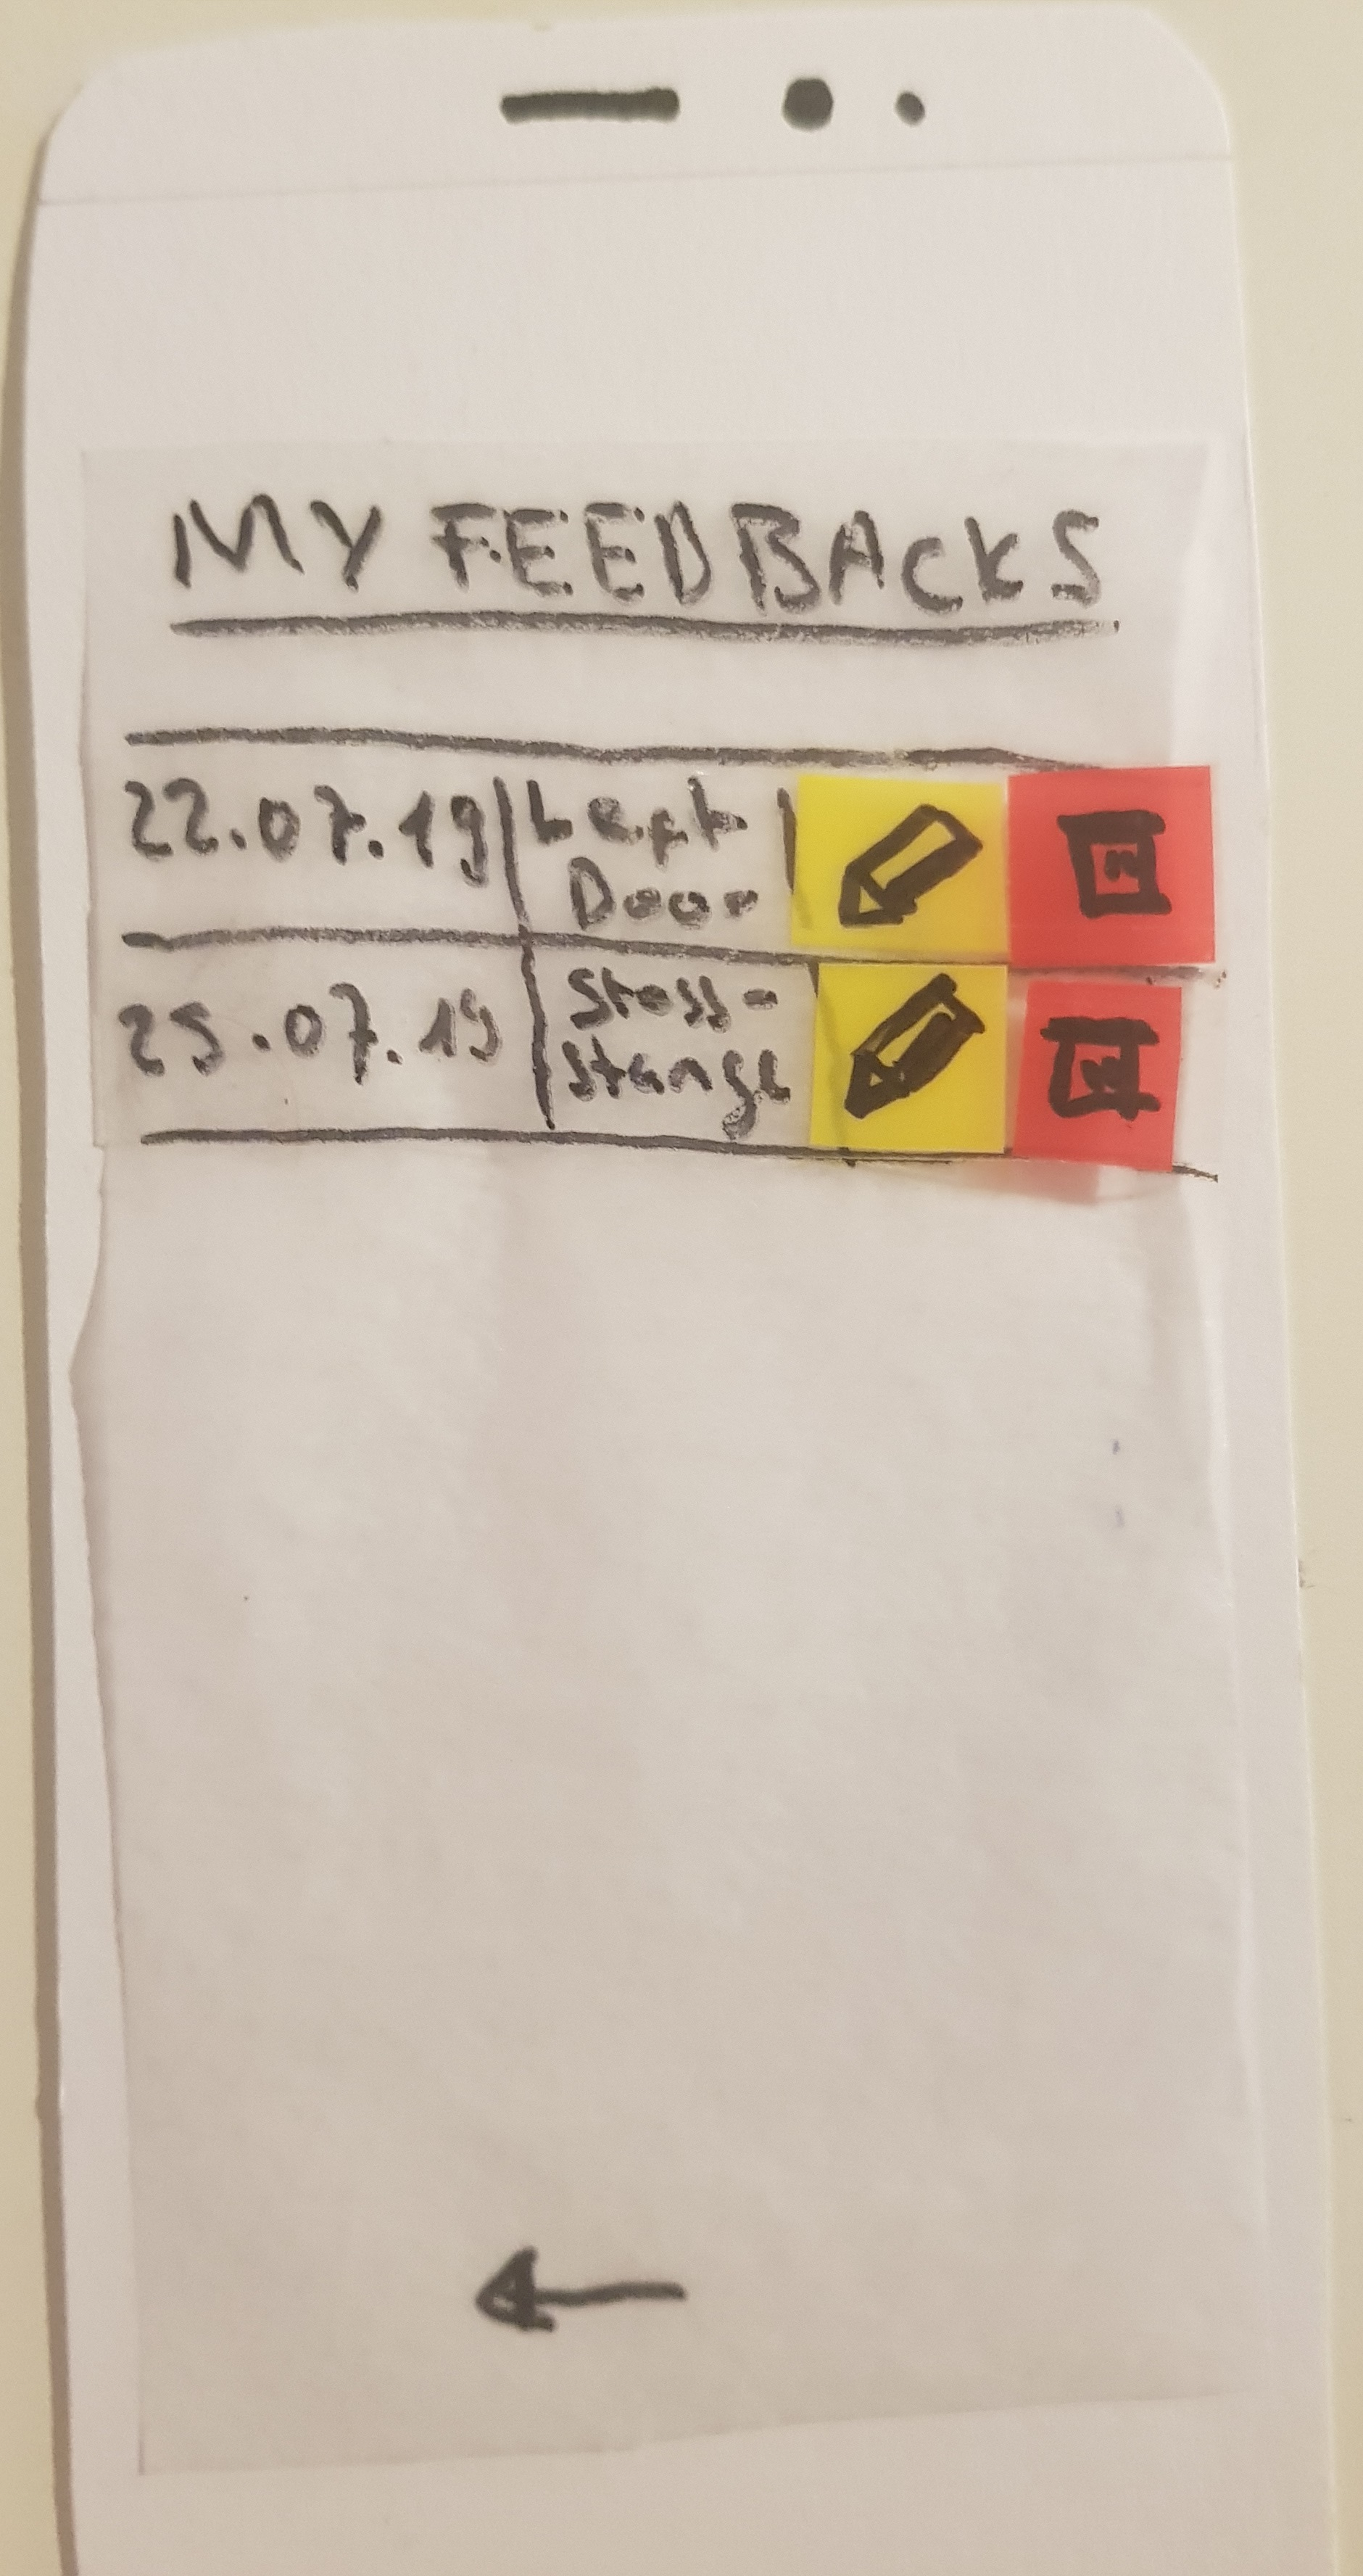
\includegraphics[width=.8\linewidth]{resources/conception/lowfi_list.jpg}
		\captionof{figure}{Papierprototyp - Listenansicht aller Feedback für die Bearbeitung und Löschung.\\Quelle: Eigene Darstellung}
		\label{fig:pplist}
	\end{minipage}
\end{figure}

Auf die in Abbildung \ref{fig:pplist} gezeigte Ansicht gelangt der Nutzer indem auf das im Startbildschirm \ref{img:pp_start} befindenden Button \textit{My Feedbacks} geklickt wird. 
Diese Ansicht beinhaltet eine Auflistung aller Feedback welche der Nutzer angelegt hat und bietet eine weitere Darstellungsform aus welcher Feedback editiert oder gelöscht werden können. 
In der Auflistung wird zu jede Feedback der Name des Produktteil sowie die Beschreibung des Feedback angezeigt. Rechts daneben werden die Buttons zum editieren und löschen angezeigt welche 
der Anwender aus der Ansicht in Abbildung \ref{img:ppeditdelete} bereits kennt.

\subsection{Objektorientierter Entwurf}\label{objentwurf}

Im folgenden werden die zu speichernden Daten für ein Feedback als ein Entitätentyp festgelegt und auf Abbildung \ref{img:entitytype} visualisiert. 

\begin{figure}[H]
	\centering
	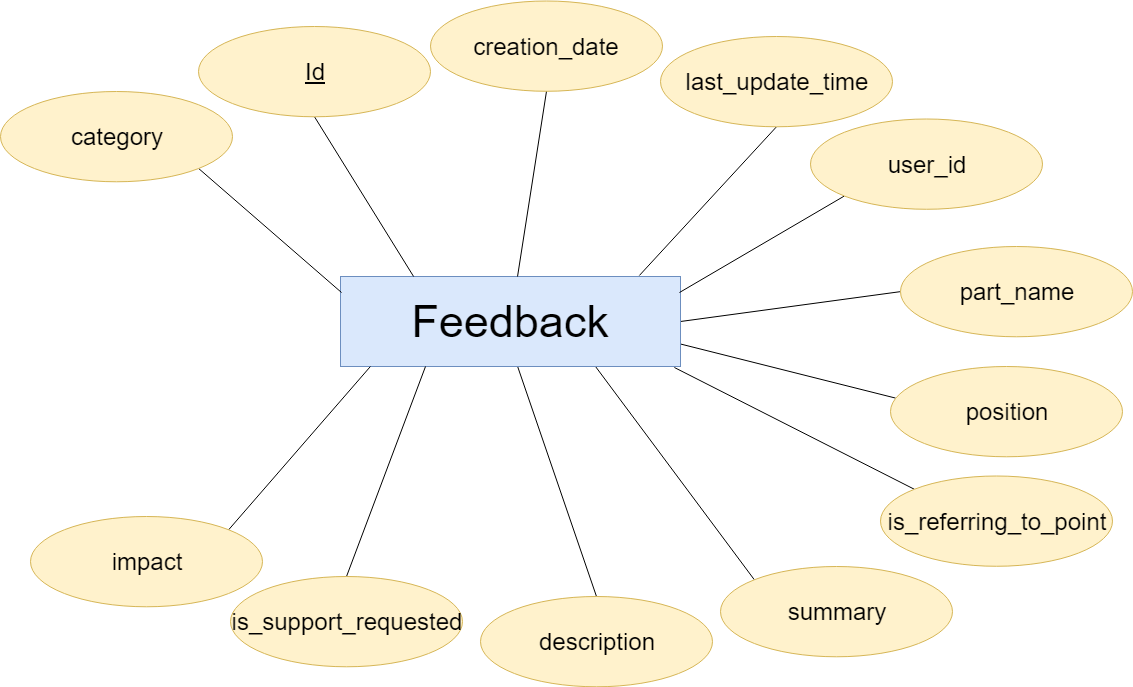
\includegraphics[width=.85\textwidth]{resources/conception/feedback_entitiy_type.png}
	\caption{Papierprototyp - Auswahl von Feedback auf dem Produkt für die Bearbeitung bzw. Löschung. \\Quelle: Eigene Darstellung}
	\label{img:entitytype}
\end{figure}

Folgend werden die einzelnen Attribute näher erläutert: 

\begin{itemize}
\item{Die \textit{Id} ist vom Datentyp Integer und bildet den Primärschlüssel. über die ein Feedback im System eindeutig identifizierbar gemacht werden soll.}
\item{Mit dem Attribut \textit{creation\_time} wird der Erstellungszeitpunkt (Zeit und Datum) festgehalten. Zeitliche Distanz bei Situated Visualization}
\item{Das Attribut \textit{last\_update\_time gibt} gibt Ausschluss darüber wann das Feedback zum letzten mal aktualisiert wurde. Zeitliche Distanz bei Situated Visualization}
\item{Über die \textit{user\_id} kann das Feedback zu einem bestimmten Nutzer zugeordnet werden.}
\item{\textit{part\_name} beihaltet den namen des Bauteils auf welches das Feedback referenziert.}
\item{Das Attribut \textit{position} ist float Array der Länge drei und wird die Postion des Ankerpunkt des der Annotation auf dem Produkt bzw. Produktteil beinhalten.}
\item{\textit{is\_referring\_to\_point} ist vom Typ Boolean und gibt Ausschluss darüber ob sich das Feedback auf die ausgewählte Stelle auf dem Produktteil oder auf das Produktteil selbst bezieht (Grad der Embeddednes)}
\item{Das Attribut \textit{description} wird die Beschreibung des Feedback beinhalten die der Nutzer eingibt. Dieser Text wird auf dem Produkt sichtbar sein.}
\item{Im Attribut \textit{impact} wird die Beschreibung für den Einfluss auf den Anwendungsfall bzw. auf den Geschäft festgehalten.}
\item{Das Attribut \textit{is\_support\_requested} gibt Ausschluss darüber ob das Feedback zeitnah vom Herstellter bearbeitet und ein Rückmeldung gegeben werden soll.}
\end{itemize}

Zuletzt wird in diesem Kapitel der Klassenentwurf des zu implementierenden Prototypen vorgestellt und in Form eines Klassendiagramms visualisiert.  
Die Klassen sind in Anlehnung an das Entwurfsmuster \textit{Model-View-Presenter} (kurz MVP, zu. dt. Modell-Ansicht-Präsentierer) entworfen. 
Abbildung \ref{img:mvp_pattern} zeigt eine schematische Darstellung diesen Entwurfsmusters. 

\begin{figure}[H]
	\centering
	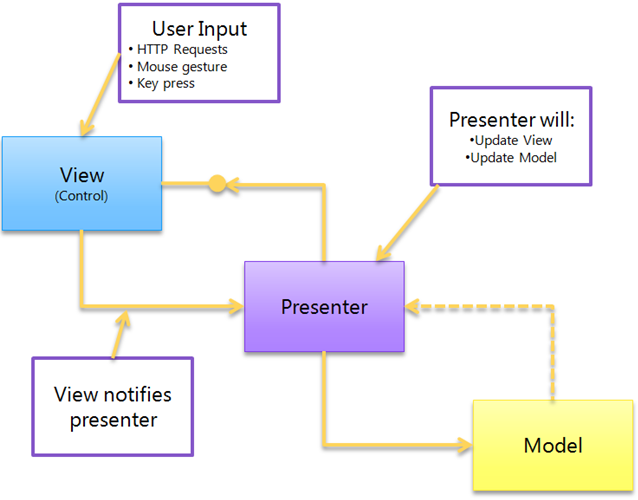
\includegraphics[width=1.0\textwidth]{resources/conception/mvp_pattern.png}
	\caption{Schematische Darstellung des MVP Entwurfmusters. \\Quelle: \cite{Valk2009}}
	\label{img:mvp_pattern}
\end{figure}

Mit diesem Muster wird die Anwendung in drei Schichten aufgeteilt:

\begin{itemize}
	\item{Die \textit{View} stellt Klassen für die Entgegennahme von Nutzereingaben über Steuerelemente der Benutzeroberfläche zur Verfügung. Benachrichtigt den \textit{Presenter} bei Ereignissen welche über gewisse Logik verarbeitet werden müssen.}
	\item{Der \textit{Presenter} binhaltet, Logik für die Verarbeitung der Nutzereingaben. Sie ist für die Synchronisierung zwischen dem \textit{Model} und der \textit{View} zuständig. Empfängt der \textit{Presenter} ein Ereignis von der \textit{View}, ruft dieser entsprechende Methoden des \textit{Models} auf um Daten zu verändern und aktualisiert anschließend die \textit{View}.}
	\item{Der \textit{Model} enthält Klassen für die Abbildung der Daten der Anwendung, Methoden für den Zugriff auf die Daten, für das Ändern der Daten sowie für die Persistenz der Daten. Das \textit{Model} hat kein Kenntnis über die \textit{View} oder den \textit{Presenter}}
\end{itemize}

Abbildung \ref{img:clasdiagramm} zeigt die Klassen des zu implementierenden Prototypen in einer Klassendiagramm visualisiert. Nachfolgend werden die dargestellten Klassen näher erläutert und den Schichten des MVP Entwurfsmusters zugeordnet: 

Die Klassen \textit{SelectionManager}, \textit{FormManager} sowie \textit{FeedbackListController} gehören bilden die View des MVP Entwurfsmusters. Die Klasse \textit{UIManger} representiert den Presenter und die Klassen 
\textit{FeedbackStorageManager}, \textit{FeedbackDB} sowie \textit{Feedback} bilden die Model Schicht.\\ 

\begin{figure}[H]
	\centering
	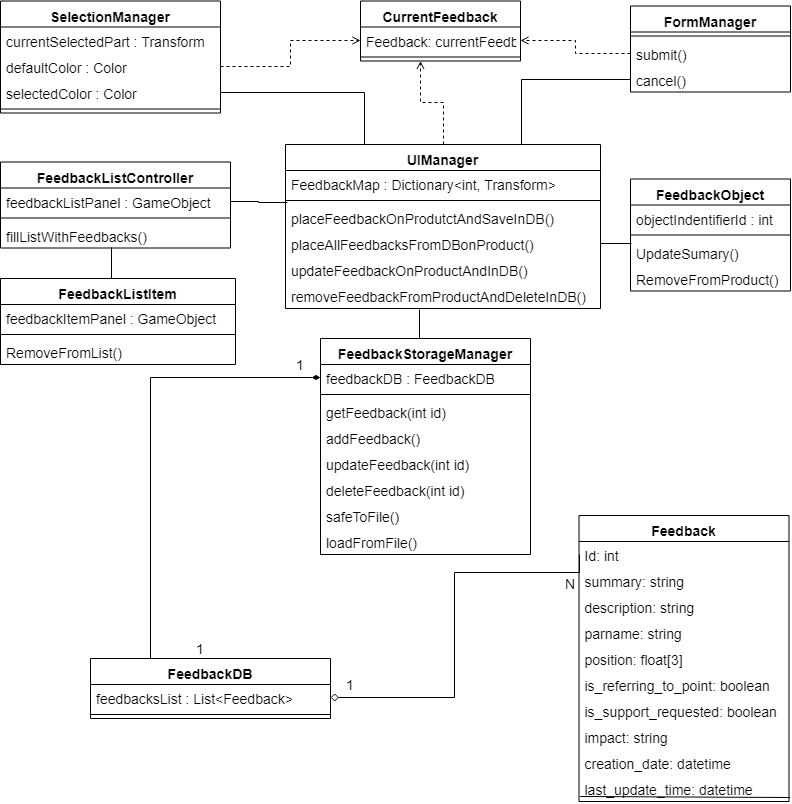
\includegraphics[width=.9\textwidth]{resources/conception/klassendiagramm.png}
	\caption{Klassendiagramm \\Quelle: Eigene Darstellung}
	\label{img:clasdiagramm}
\end{figure}

Nachfolgend werden die Klassen näher erläutert: 

\vspace{4mm}
\begin{tabularx}{\textwidth}{l X}
	\vspace{1mm}\textbf{SelectionManager} & Nimmt Nutzereingaben über die über die Touchscreen Benutzeroberfläche kommen entgegen und ist für das Zeigen auf dem Produkt, in Fokus rücken ausgewählter Produktteile sowie das Informieren des UIManagers über Selektion von Stelle auf auf dem Produkt oder bestehender Feedback zuständig.\\
	\vspace{1mm}\textbf{FormManager} & Ist für die Koordinierung der Steuerelemente auf des Eingabeformulars (Abbildung \ref{fig:test1}), der Validierung von Nutzereingaben, sowie das Informieren des UIManagers über Ereignisse (Feedback Anlegen Button gedrück oder Cancel Button gedrückt) zuständig. \\
	\vspace{1mm}\textbf{FeedbackListController}  & Ist für die Koordinierung der Listenansicht (Abbildung \ref{fig:pplist}) für alle Feedback eines Nutzers zuständig.\\
	\vspace{1mm}\textbf{CurrentFeedback}  & Ein Singleton Instanz\footnote{Als Singleton werden Klassen bezeichnet welche nach dem Entwurfsmuster Singleton implementiert sind. Von diesen Klassen kann nur eine einzige Instanz in der Applikation instanziiert werden.} welches Informationen über das aktuell anzulegende, noch nicht im Model gespeichertes Feedback beinhaltet. Die Klassen SelectionManager sowie FormManager greifen auf diese Klasse zu um Informationen zu aktualisieren. Die UIManager Klasse greift auf diese Klasse zu um aus den enthaltenen Informationen im Model ein neues Feedback anzulegen.\\
	\vspace{1mm}\textbf{FeedbackObject}  & Diese Klasse wird als Skript an eine Annotation welches in Unity als ein Prefab angelegt wird hinzugefügt und hat zwei Aufgaben. Sie einhält eine Id über die ein Annotation auf dem Produkt (eine Instanz in der View) eindeutig identifizierbar gemacht wird. Diese Id wird mit der Id aus dem Datenmodel \ref{img:entitytype} übereinstimmen. Des weiteren wird dieses Skript Methoden für die Steuerung der Annotation verfügen (z. B. zum Nutzer rotieren, sich vom Produkt entfernen)\\
	\vspace{1mm}\textbf{FeedListItem} & Diese Klasse wird als ein Skript an jede Listeneintrag welche ein Feedback in der Listenansicht (Abbildung \ref{fig:pplist}) repräsentieren angefügt. Diese Klasse verfügt über Methoden für die Enfernung des Listeneintrags aus der Listenansicht oder die Aktualisierung. \\
	\vspace{1mm}\textbf{UIManager} & Enthält Methoden für die Entgegennahme von Ereignisse die von den Ansichten kommen (SelectionManager, FormManager) sowie die Logik um auf diese Ereignisse zu reagieren. Sie verfügt über Methoden wie das Anlegen eines neuen Feedbacks über die Nutzung von Methoden die der FeedbackStorageManager zur Verfügung stellt, sowie das Platzieren eines Feedbacks oder die Platzierung aller Feedbacks aus der Datenbank auf dem Produkt. \\
	\vspace{1mm}\textbf{FeedbackStorageManager} & Diese Klasse stellt Methoden für den Zugriff auf die Datenbank (FeedbackDB) zur verfügung und enthält Methoden zum anlegen, verändern oder löschen von Feedback aus der Datenbank. Sie enthält zudem Methoden für die Serialisierung\footnote{Serialisierung  beschreibt die Umwandulung eines Objektes in eine Folge von Bytes. Quelle: https://www.it-visions.de/glossar/alle/3468/Deserialisierung.aspx [Letzter Zugriff: 09.09.2019]} und Deserialisierung\footnote{Deserialisierung beschreiben die den Vorgang bei welcher aus eienr Folge von Bystes ein bestimmtes Objekt aus der objektorientierten Programmierung erzeugt wird. Quelle: https://www.it-visions.de/glossar/alle/3468/Deserialisierung.aspx [Letzter Zugriff: 09.09.2019]} der Daten zum laden und lesen aus einer Datei zur Verfügung. \\
	\vspace{1mm}\textbf{FeedbackDB} & Kapselt die Daten welche in Form einer Liste gespeichert werden. \\
	\vspace{1mm}\textbf{Feedback} & Repräsentiert ein Feedback as Datenmodel im System.\\
\end{tabularx}
